\newcommand{\installerTagResultsAucTable}{
    \begin{table}[H]
        \centering
        \begin{tabular}{|p{2,8cm}||p{2,8cm} p{2,8cm} p{2,8cm}|}
            \hline
            Installer Tag & ALOHA & Joint Embedding & Proposed Model \\
            \hline
            AUC-ROC & \textBF{0.976$\pm$0.001} & 0.971$\pm$0.002 & 0.975$\pm$0.003 \\
            \hline
        \end{tabular}
        \caption{AUC-ROC (Area Under Curve) of the different models for the \textbf{Installer Tag} prediction task. Results were aggregated over \textBF{3} training runs with different weight initializations and minibatch orderings. Best results are shown in \textbf{bold}.} \label{tab:installerTag_auc}
    \end{table}
}

\newcommand{\installerTagResultsAtFprTable}{
    \begin{center}
        \begin{longtable}[c]{|p{3,2cm}||p{1,8cm} p{1,8cm} p{1,8cm} p{1,8cm} p{1,8cm}|}
            \hline
            Installer Tag & \multicolumn{5}{c|}{{FPR}} \\
            & $10^{-5}$ & $10^{-4}$ & $10^{-3}$ & $10^{-2}$ & $10^{-1}$ \\
            \hline
            \endfirsthead

            \caption*{\raggedright ...continued from previous page} \\
            \hline
            Installer Tag & \multicolumn{5}{c|}{\textbf{FPR}} \\
            & $10^{-5}$ & $10^{-4}$ & $10^{-3}$ & $10^{-2}$ & $10^{-1}$ \\
            \hline
            \endhead

            \caption*{\raggedleft ...continued on next page} \\
            \endfoot

            \caption{Mean and standard deviation results (TPR, Accuracy, Recall, Precision and F1-Score) of the different models for the \textbf{Installer Tag} prediction task at different \textbf{FPR}s (\textit{False Positive Rates}). Results were aggregated over \textBF{3} training runs with different weight initializations and minibatch orderings. Best results are shown in \textbf{bold}. Under \textbf{TPR} results are also presented the percentage reduction in mean detection error and in ROC curve standard deviation introduced by the \textit{Proposed Model} with respect to both \textit{ALOHA} model and \textit{Joint Embedding}.} \label{tab:installerTag_results_at_fpr} \\
            \endlastfoot

            \multicolumn{6}{|c|}{\textbf{TPR}} \\
            \hline
            ALOHA & 0.176$\pm$0.012 & 0.252$\pm$0.005 & 0.380$\pm$0.002 & 0.755$\pm$0.009 & \textBF{0.949$\pm$0.007} \\
            Joint Embedding & \textBF{0.202$\pm$0.024} & \textBF{0.298$\pm$0.007} & 0.478$\pm$0.007 & 0.762$\pm$0.026 & 0.942$\pm$0.005 \\
            Proposed Model & 0.190$\pm$0.008 & 0.266$\pm$0.024 & \textBF{0.480$\pm$0.028} & \textBF{0.766$\pm$0.034} & 0.938$\pm$0.016 \\
            \hline
            Error Reduction wrt \newline ALOHA & 1.7\% & 1.9\% & 16.1\% & 4.5\% & -21.6\% \\
            Error Reduction wrt \newline Joint Embedding & -1.5\% & -4.6\% & 0.4\% & 1.7\% & -6.9\% \\
            \hline
            Std Reduction wrt \newline ALOHA & 33.3\% & -380.0\% & -1300.0\% & -277.8\% & -128.6\% \\
            Std Reduction wrt \newline Joint Embedding & 66.7\% & -242.9\% & -300.0\% & -30.8\% & -220.0\% \\
            \hline
            \multicolumn{6}{|c|}{\textbf{Accuracy}} \\
            \hline
            ALOHA & 0.985$\pm$0.000 & \textBF{0.987$\pm$0.000} & 0.988$\pm$0.000 & \textBF{0.986$\pm$0.000} & \textBF{0.901$\pm$0.000} \\
            Joint Embedding & \textBF{0.986$\pm$0.000} & \textBF{0.987$\pm$0.000} & \textBF{0.990$\pm$0.000} & \textBF{0.986$\pm$0.000} & \textBF{0.901$\pm$0.000} \\
            Proposed Model & \textBF{0.986$\pm$0.000} & \textBF{0.987$\pm$0.000} & 0.990$\pm$0.001 & 0.986$\pm$0.001 & \textBF{0.901$\pm$0.000} \\
            \hline
            \multicolumn{6}{|c|}{\textbf{Recall}} \\
            \hline
            ALOHA & 0.176$\pm$0.012 & 0.252$\pm$0.005 & 0.380$\pm$0.002 & 0.755$\pm$0.009 & \textBF{0.949$\pm$0.007} \\
            Joint Embedding & \textBF{0.202$\pm$0.024} & \textBF{0.298$\pm$0.007} & 0.478$\pm$0.007 & 0.762$\pm$0.026 & 0.942$\pm$0.005 \\
            Proposed Model & 0.190$\pm$0.008 & 0.266$\pm$0.024 & \textBF{0.480$\pm$0.028} & \textBF{0.766$\pm$0.034} & 0.938$\pm$0.016 \\
            \hline
            \multicolumn{6}{|c|}{\textbf{Precision}} \\
            \hline
            ALOHA & \textBF{0.997$\pm$0.000} & 0.979$\pm$0.000 & 0.874$\pm$0.001 & 0.578$\pm$0.003 & \textBF{0.147$\pm$0.001} \\
            Joint Embedding & \textBF{0.997$\pm$0.000} & \textBF{0.982$\pm$0.000} & \textBF{0.896$\pm$0.001} & 0.579$\pm$0.008 & 0.146$\pm$0.001 \\
            Proposed Model & \textBF{0.997$\pm$0.000} & 0.980$\pm$0.002 & 0.896$\pm$0.005 & \textBF{0.581$\pm$0.011} & 0.145$\pm$0.002 \\
            \hline
            \multicolumn{6}{|c|}{\textbf{F1 Score}} \\
            \hline
            ALOHA & 0.299$\pm$0.018 & 0.401$\pm$0.006 & 0.529$\pm$0.002 & 0.655$\pm$0.005 & \textBF{0.254$\pm$0.002} \\
            Joint Embedding & \textBF{0.336$\pm$0.032} & \textBF{0.457$\pm$0.008} & 0.624$\pm$0.006 & 0.658$\pm$0.015 & 0.252$\pm$0.001 \\
            Proposed Model & 0.318$\pm$0.011 & 0.417$\pm$0.029 & \textBF{0.625$\pm$0.025} & \textBF{0.661$\pm$0.020} & 0.251$\pm$0.004 \\
            \hline
        \end{longtable}
    \end{center}
}

\newcommand{\installerTagResultsSummaryTable}{
    \begin{table}[H]
        \centering
        \begin{tabular}{|p{3,2cm}||p{1,8cm} p{1,8cm} p{1,8cm} p{1,8cm} p{1,8cm}|}
            \hline
            \multicolumn{6}{|c|}{Installer Tag (at FPR $=1\%$)} \\
            \hline
            Model & TPR & Accuracy & Precision & Recall & F1 score \\
            \hline
            ALOHA & 0.755$\pm$0.009 & \textBF{0.986$\pm$0.000} & 0.578$\pm$0.003 & 0.755$\pm$0.009 & 0.655$\pm$0.005 \\
            Joint Embedding & 0.762$\pm$0.026 & \textBF{0.986$\pm$0.000} & 0.579$\pm$0.008 & 0.762$\pm$0.026 & 0.658$\pm$0.015 \\
            Proposed Model & \textBF{0.766$\pm$0.034} & 0.986$\pm$0.001 & \textBF{0.581$\pm$0.011} & \textBF{0.766$\pm$0.034} & \textBF{0.661$\pm$0.020} \\
            \hline
        \end{tabular}
        \caption{Summary of the mean and standard deviation results of the different models for the \textbf{Installer Tag} prediction task at \textbf{FPR} $=1\%$. Results were aggregated over \textBF{3} training runs with different weight initializations and minibatch orderings. Best results are shown in \textbf{bold}.} \label{tab:installerTag_result_summary}
    \end{table}
}

\newcommand{\installerTagRocAloha}{
    \begin{figure}[H]
        \vspace*{-0.5cm}
        \centering
        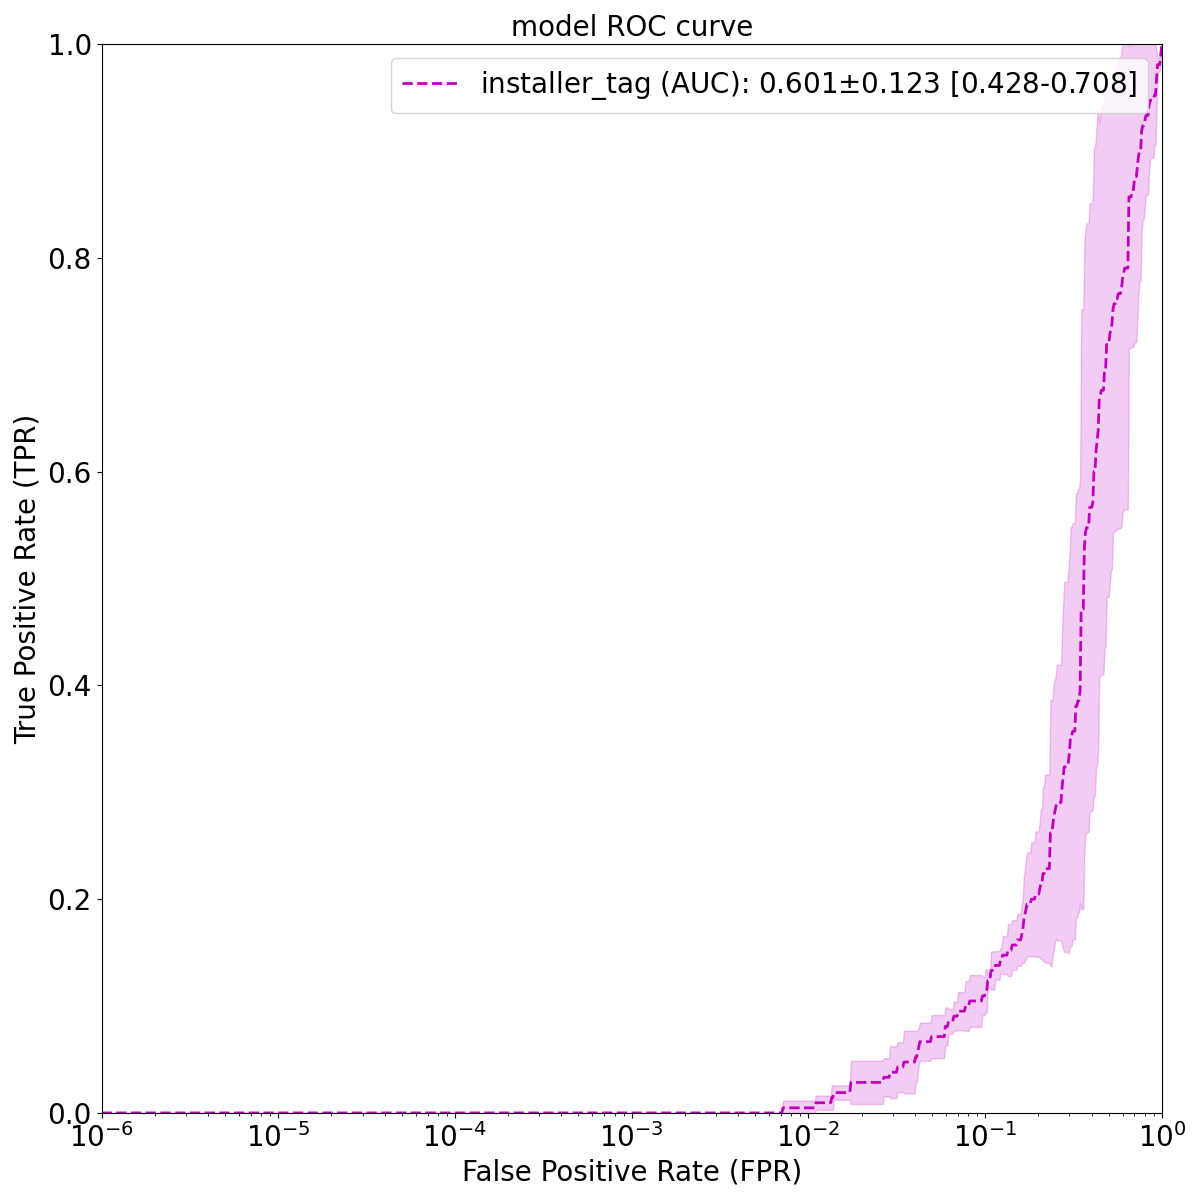
\includegraphics[width=0.6\textwidth]{./results/installer_tag_roc_aloha.png}
        \vspace*{-0.2cm}
        \caption{ROC curve and AUC statistics of \textBF{ALOHA} model for the \textbf{Installer Tag}. The line represents the \textit{mean} TPR at a given FPR, while the shaded region represents the \textit{standard deviation}. Statistics were computed over \textBF{3} training runs, each with random parameter initialization.}
        \label{fig:installerTagRocAloha}
    \end{figure}
}

\newcommand{\installerTagRocJointEmbedding}{
    \begin{figure}[H]
        \vspace*{-0.5cm}
        \centering
        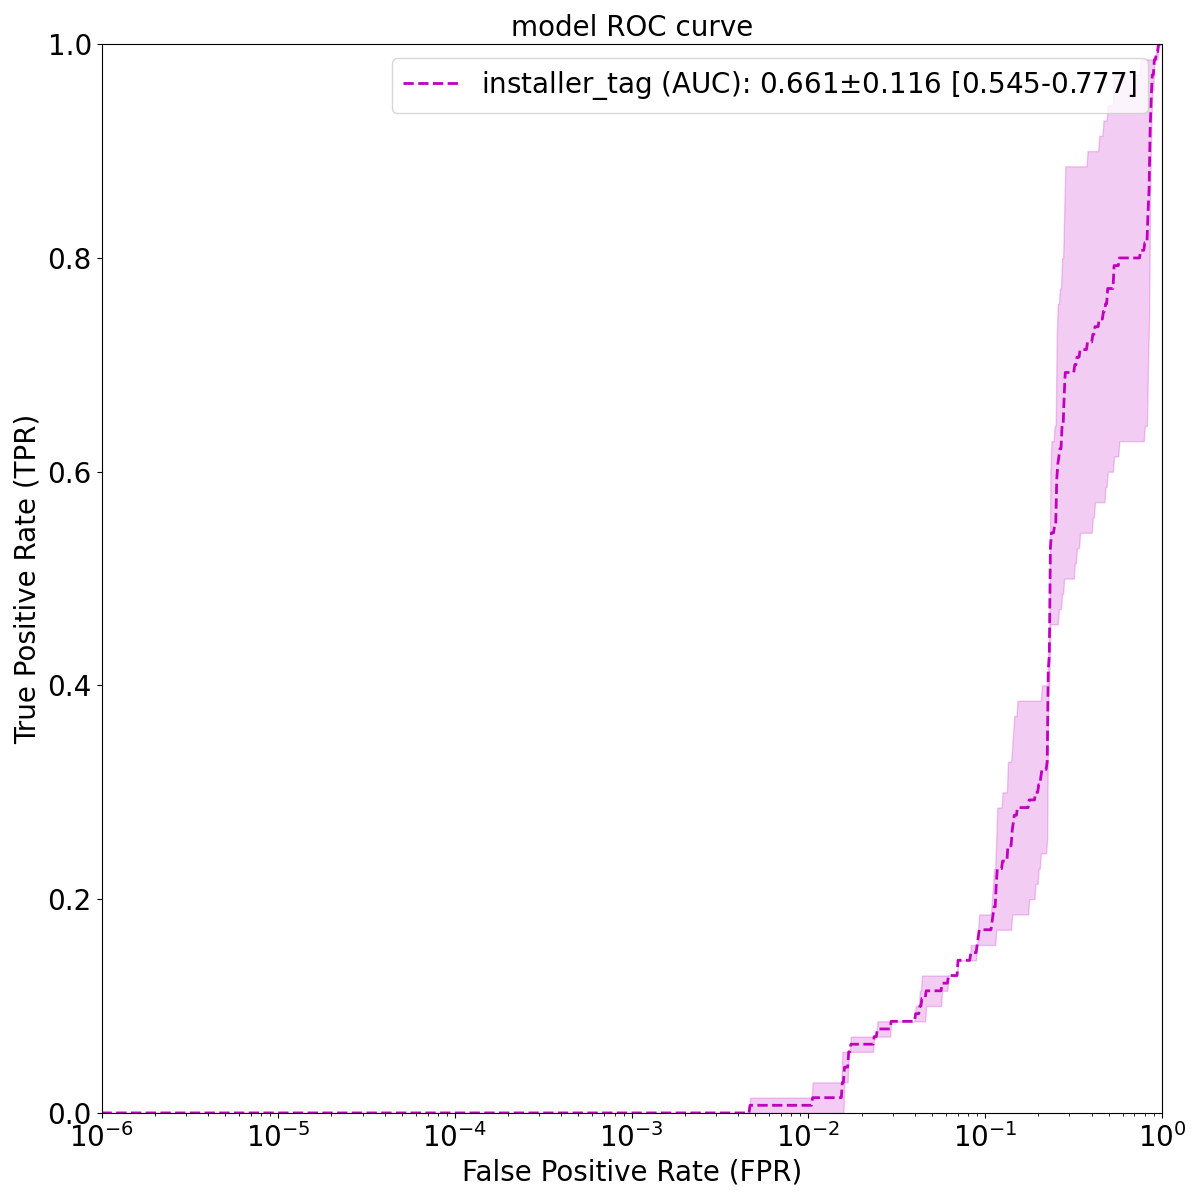
\includegraphics[width=0.6\textwidth]{./results/installer_tag_roc_jointEmbedding.png}
        \vspace*{-0.2cm}
        \caption{ROC curve and AUC statistics of \textBF{Joint Embedding} model for the \textbf{Installer Tag}. The line represents the \textit{mean} TPR at a given FPR, while the shaded region represents the \textit{standard deviation}. Statistics were computed over \textBF{3} training runs, each with random parameter initialization.}
        \label{fig:installerTagRocJointEmbedding}
    \end{figure}
}

\newcommand{\installerTagRocProposedMethod}{
    \begin{figure}[H]
        \vspace*{-0.5cm}
        \centering
        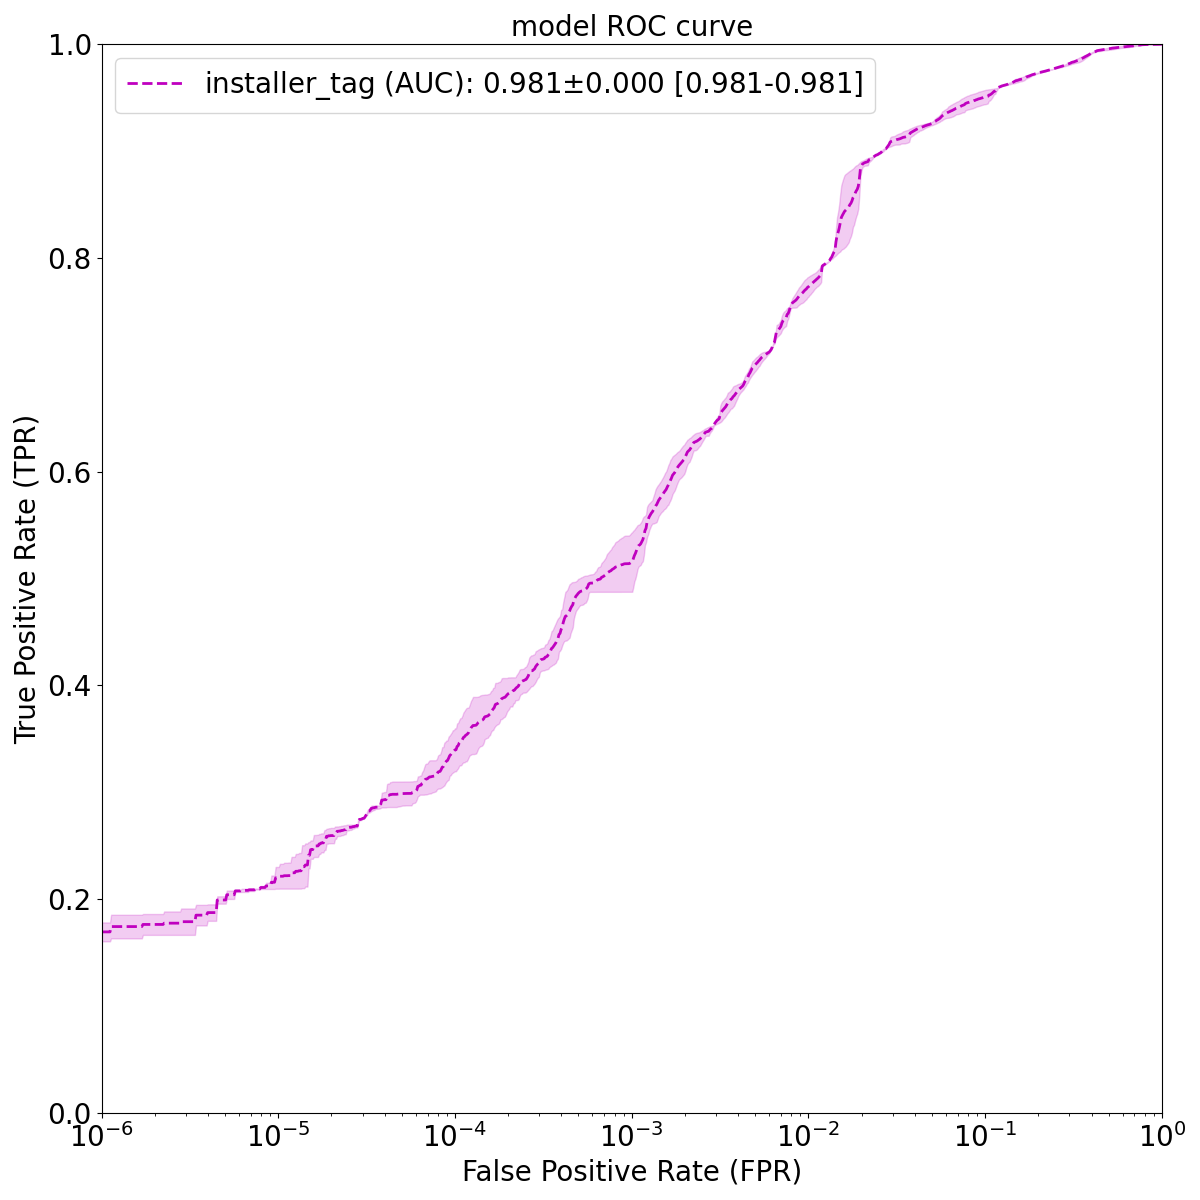
\includegraphics[width=0.6\textwidth]{./results/installer_tag_roc_proposedModel.png}
        \vspace*{-0.2cm}
        \caption{ROC curve and AUC statistics of \textBF{Proposed Model} for the \textbf{Installer Tag}. The line represents the \textit{mean} TPR at a given FPR, while the shaded region represents the \textit{standard deviation}. Statistics were computed over \textBF{3} training runs, each with random parameter initialization.}
        \label{fig:installerTagRocProposedModel}
    \end{figure}
}
